\setlength{\columnsep}{3pt}
\begin{flushleft}
	\begin{itemize}
		\item \textbf{A process is a program running} in the Linux system \textbf{using memory \& CPU}.
		\item A Linux process is also called \textbf{service or daemon}.
		\item Every process has many details associated with it, some of them are:
		\begin{itemize}
			\item Process ID
			\item Process name
			\item A program associated with it
			\item Process state
			\item User owning the process
		\end{itemize}
		
		\begin{figure}[h!]
			\centering
			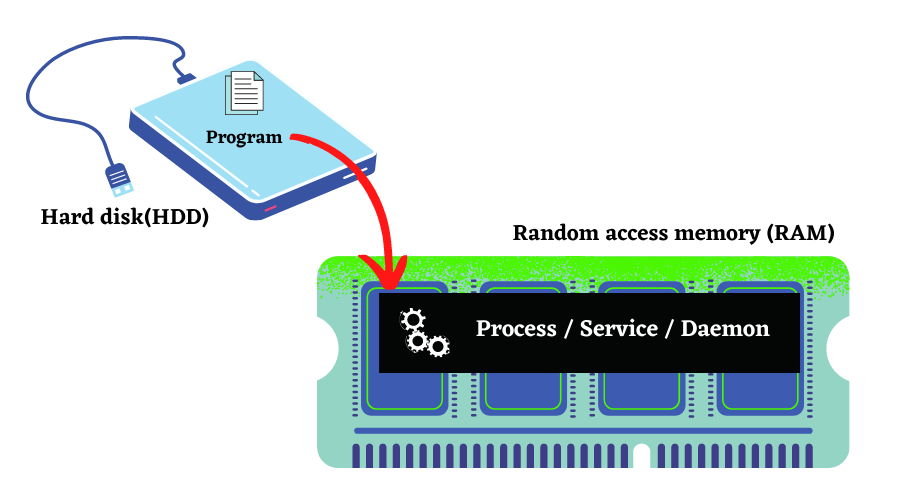
\includegraphics[scale=.55]{content/chapter12/images/process.png}
			\caption{Process/Service/Daemon}
			\label{fig:process}
		\end{figure}
		
		\item Keeping unused Linux process running in the system is \textbf{a waste of RAM \& CPU}.
		\item Unused process can expose your system to \color{red}security threat.
	\end{itemize}
\end{flushleft}

\newpage


